\section{Theorie}
\label{sec:Theorie}
Zunächst wird ein einzelnes Fadenpendel mit der angehängten Masse $m$ und der Pendellänge $l$ betrachtet.
Zudem wird angenommen, dass die Pendelaufhängung reibungsfrei sei und Däpfungseffekte werden als vernachlässigbar klein erachtet.
Wird das Pendel ausgelenkt, wirkt die Gewichtskraft der Auslenkung entgegen und verursacht ein rückstellendes Drehmoment $M=D_{\mathrm{p}}\cdot \phi$.
Hierbei ist $D_{\mathrm{p}}$ die Winkelrichtgröße und $\phi$ der Auslenkwinkel.
Die Gewichtskraft $F_{\mathrm{G}}=J\cdot\ddot\phi$ ergibt sich aus $F_{\mathrm{G}}=m\cdot a$, indem die Beschleunigung $a$ durch die Winkelbeschleunigung ersetzt wird.
Zudem wird beachtet, dass die Pendelmasse ausgedehnt ist. Somit wird das Massenträgheitsmoment $J$ eingeführt.
Für kleine Winkel kann die Kleinwinkelnäherung, $\sin{\phi}=\phi$ verwendet werden und es ergibt sich die Bewegungsgleichung
\begin{equation}
	J\cdot \ddot\phi=-D_{\mathrm{p}}\phi \text{.}
\end{equation}

Durch die Lösung der Bewegungsgleichung wird eine harmonische Schwingung beschrieben. Die Schwingungsfrequenz ergibt sich hierbei zu
\begin{equation}
	\omega=\sqrt{\frac{D_{\mathrm{p}}}{J}}=\sqrt{\frac{g}{l}} \text{.}
\end{equation}
Da sich die Schwingungsdauer direkt aus der Schwingungsfrequenz ergibt, hängt diese also für kleine Auslenkunden weder von der Pendelmasse, noch vom Auslenkwinkel $\phi$ ab.

Werden zwei Pendel mit identischer Pendellänge und-masse durch eine Feder gekoppelt, wirkt ein zusätzliches Moment $D_{\mathrm{F}}$ auf die beiden Pendel.
Dabei ist $D_{\mathrm{F}}$ abhängig von der Dehnung der Feder. Diese ergibt sich hier über die Auslenkwinkel $\phi_{\mathrm{i}}$ der beiden Pendel.
Aufgrund der Kopplung durch die Feder lässt sich die Bewegung somit durch ein System gekoppelter Differentialgleichungen
\begin{gather}
	J\cdot \ddot \phi_1 + D_{\mathrm{p}} \phi_1=D_{\mathrm{F}}(\phi_2-\phi_1)\text{,}\\
	J\cdot \ddot \phi_2 + D_{\mathrm{p}} \phi_2=D_{\mathrm{F}}(\phi_1-\phi_2)\text{.}
\end{gather}
beschreiben.
Durch eine geeignete Wahl der Winkel lässt sich das System entkoppeln und als Überlagerung der Einzelschwingungen der Pendel formulieren.
Die Lösungen der entkoppelten Differentialgleichungen sind wiederum harmonische Schwingungen mit der Kreisfrequenz $\omega_{\mathrm{i}}$ und dem Auslenkwinkel $\alpha_{\mathrm{i}}$
Je nach Anfangsbedingungen des Systems, also Anfangsauslenkung und Anfangswinkelgeschwindigkeit, werden verschiedene Schwingungsarten unterschieden.
%änder bloß nichts an den Bildgrößen, das ist superkacke mit dem wrapfigure ding
\subsection{Gleichsinnige Schwingung}
\FloatBarrier
\begin{wrapfigure}[13]{r}{0.4\textwidth}
	\centering
	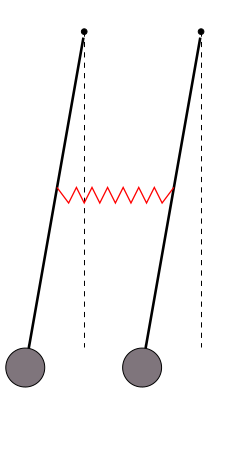
\includegraphics[width=0.4\linewidth]{Bilder/gleichphasig.png}
	\caption{Gleichsinnige Schwingung \cite{Anleitung}.}
	\label{fig:gleich}
\end{wrapfigure}
\FloatBarrier
Sind zu Beginn beide Pendel um den gleichen Winkel, also $\alpha_1=\alpha_2$ ausgelenkt, ist die Feder nicht gespannt und verursacht daher kein zusätzliches Moment.
Somit ist die Schwingungsfrequenz und die Schwingungsdauer identisch mit den Werten für ein einzelnes Pendel.
Für die Schwingungsfrequenz ergibt sich somit
\begin{equation}
	\omega_{\mathrm{+}}=\sqrt{\frac{g}{l}}
\end{equation}
und für die Schwingungsdauer gilt
\begin{equation}
	T_{\mathrm{+}}=2\pi\cdot\sqrt{\frac{l}{g}} \text{.}
\end{equation}

\subsection{Gegensinnige Schwingung}
\FloatBarrier
\begin{wrapfigure}[12]{r}{0.4\textwidth}
	\centering
	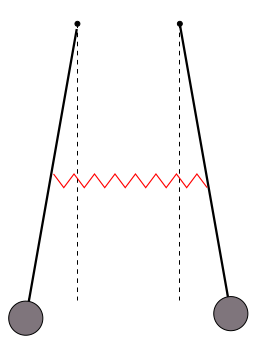
\includegraphics[width=0.4\linewidth]{Bilder/gegenphasig.png}
	\caption{Gegensinnige Schwingung \cite{Anleitung}.}
	\label{fig:gegen}
\end{wrapfigure}
\FloatBarrier
Sind beide Pendel gegengleich ausgelenkt, gilt also für die Auslenkwinkel $\alpha_1=-\alpha_2$, so übt die Kopplungsfeder auf beide Pendel die entgegegen gesetzt gleichgroße Kraft aus.
Hierdurch ergibt sich eine symmetrische Schwingung mit der Schwingungsfrequenz
\begin{equation}
	\omega_{\mathrm{-}}=\sqrt{\frac{g}{l}+\frac{2 K}{l}}
\end{equation}
und die Schwingungsdauer
\begin{equation}
	T_{\mathrm{-}}=2\pi\cdot\sqrt{\frac{l}{g+2K}} \text{.}
\end{equation}
Die Kopplungskonstante der Feder ist hierbei $K$.
\subsection{Gekoppelte Schwingung}
Werden beide Pendel unterschiedlich weit ausgelenkt, also zum Beispiel $\alpha_1=0$ und $\alpha_2 \neq 0$ lässt sich eine Schwebung beobachten.
Diese entsteht, indem das zuerst ausgelenkte über die Kopplung durch die Feder nach und nach das andere Pendel in Schwingung versetzt, indem die gesamte Energie des zuvor ausgelenkten Pendel nach und nach auf das zu Beginn ruhende Pendel übertragenn wird.
Die Schwingungsamplitude des zu Beginn ausgelenkten Pendels nimmt nun im gleichen Maße ab, wie die des zuvor ruhenden Pendel zunimmt.
Schließlich kommt das zu Beginn ausgelenkte Pendel zur Ruhe und der Vorgang wiederholt sich.
Die Zeit zwischen zwei Stillständen eines Pendels wird hierbei als \textbf{Schwebung} bezeichnet.
\FloatBarrier

\begin{wrapfigure}[12]{r}{0.4\textwidth}
	\centering
	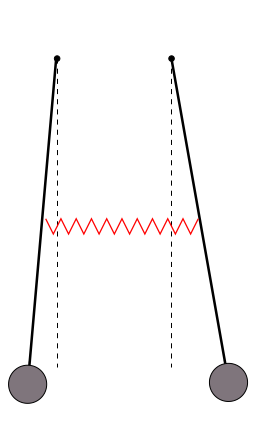
\includegraphics[width=0.4\linewidth]{Bilder/gekoppelt.png}
	\caption{Gekoppelte Pendel \cite{Anleitung}.}
	\label{fig:schwebe}

\end{wrapfigure}
\FloatBarrier
Die Schwebungsdauer $T_{\mathrm{S}}$ und die Schwebungsfrequenz $\omega_{\mathrm{S}}$ lassen sich hierbei über die bereits betrachteten Schwingungsdauern-und -frequenzen der gegen-und gleichsinnigen Schwingung wie folgt bestimmen
\begin{gather}
	T_{\mathrm{S}}=\frac{T_{\mathrm{+}}\cdot T_{\mathrm{-}}}{T_{\mathrm{+}}-T_{\mathrm{-}}} \text{,}\\
	\omega_{\mathrm{S}}=\omega_{\mathrm{+}}-\omega{\mathrm{-}} \text{.}
\end{gather}
Der \textbf{Kopplungsgrad} der Feder $\kappa$ wird definiert als
\begin{equation}
	\kappa=\frac{\omega_{\mathrm{-}}^2-\omega_{\mathrm{+}}^2}{\omega_{\mathrm{-}}^2+\omega_{\mathrm{+}}^2}=\frac{T_{\mathrm{+}}^2-T_{\mathrm{-}}^2}{T_{\mathrm{+}}^2+T_{\mathrm{-}}^2}
\end{equation}
